\chapter{Properties of Single-Wall Carbon Nanotubes}

\section{Introduction}
{\color{red}UNFINISHED} Carbon nanotubes are 1-D structures meaning that electrons are confined in a single dimension. They exist in terms of many chiralities, some are semiconducting and others are metallic \cite{soavi2016ultrafast}. Interesting because they let us explore the physics of 1-D structures. Due to the higher degree of confinement with respect to convention 3-D structures, different phenomena may occur.



\section{Carbon Nanotube Chiralities}

{\color{red}UNFINISHED} Carbon nanotubes are basically rolled up graphene sheets. Countless ways of rolling up a graphene sheet into cylindrical structures. Depending on the arrangement of the crystal lattice structure as well as the tube diameter, carbon nanotubes can behave as either metals or semiconductors \cite{ando1997excitons, nanot2012optoelectronic}. Hence, nanotubes described using so-called chiral vectors.

\subsection{Definition of the Chiral Vector $\vec{C_h}$}



 Species of carbon nanotubes are denoted using a set of indices ($m$,$n$). These integers $m$ and $n$ define the chiral vector $\vec{C_h }$ expressed as 
\begin{equation}
	\vec{C_h} = n {\vec{a_1}} + m {\vec{a_2}} \equiv (m,n)
\end{equation}

where $\vec{a_1}$ and $\vec{a_2}$ represent the lattice basis vectors of the 2D graphene sheet as shown in Figure \ref{fig:chiral_vectors} \cite{nanot2013single}. This chiral vector $\vec{C_h}$ yields the nanotube diameter $d_t$ via the expression



\begin{equation}
	d_t = \dfrac{|\vec{C_h}|}{\pi} = \dfrac{a_{C-C}}{\pi}\sqrt{3(m^2 + mn + n^2)},
\end{equation} 

where $a_{C-C} \approx$ \SI{1.44}{\angstrom} defines the nearest-neighbor distance between carbon atoms in graphene \cite{nanot2013single}.  

\begin{figure}[H]
	\centering
	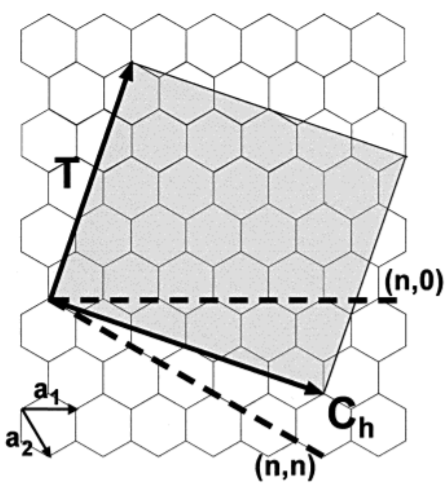
\includegraphics[scale=1]{images/chapter_optical_props/chiral_vectors_sheet.png}
	\caption{{\color{red}UNFINISHED CAPTION}}
	\label{fig:chiral_vectors}
\end{figure}

\subsection{Chiralities of Semiconducting and Metallic Nanotubes}
The chiral vector $\vec{C_h}$ also provides the means of distinguishing between semiconducting and metallic nanotubes. In general, (n,n) carbon nanotubes constitute the set of all metallic nanotubes \cite{nanot2012optoelectronic}. All (n,m) nanotubes where $n-m = 3j$ ($j > 0$) comprise a set of small-gap ($\sim1 - 100$ meV band gap energy) semiconductors \cite{nanot2012optoelectronic}. The remaining nanotubes outside of these two categories include medium-gap semiconductors ($\sim0.5 - 1$ eV band gap energy) \cite{nanot2012optoelectronic}.


\section{Electronic Properties}

Chirality vector a consequence of 1-D character of carbon nanotubes. 1-D structures expected 
{\color{red}UNFINISHED} Strong electron-electron interactions largely influence the binding energies of quasi-particles known as excitons that form after the creation of an electron-hole pair \cite{koch2006semiconductor}. Excitons represent hydrogen-like particles composed of a negatively-charged electron bound to a positively-charged hole \cite{koch2006semiconductor}. Similar to hydrogen atoms, they also possess their own set of analagous optical transitions \cite{koch2006semiconductor}. In an ideal 1-D material, theory predicts that excitons have an infinite binding energy. This alone foreshadows the dominance of excitons in the optical properties of carbon nanotubes \cite{ando2005theory}. 

\subsection{Band Structure}

Start with band structure of graphene. Assert periodic boundary conditions to get new band structure. Metallic nanotubes possess Dirac cone as well as subbands. Semiconducting nanotubes only have subbands.


{\color{red}UNFINISHED} In a simple tight-binding picture, density of states consists of Van-Hove singularities in both the valence and conduction bands. Here, each Van-Hove singularity associated with a sub-band. This model however ignores the effects of electron-electron interactions and thereby does not account for the effects of quantum confinement \cite{weismanKonoBook}. Indeed, the inclusion of electron-electron interactions into this picture yields a new electronic structure in which free electrons play a minimal role.

\subsection{Suppression of the Free Electron Continuum}

Both theoretical and experimental studies demonstrate that the strong quantum confinment of nanotubes effectively suppresses the density of states of any free electron continuum.  
 
 \begin{figure}[H]
 	\centering
 	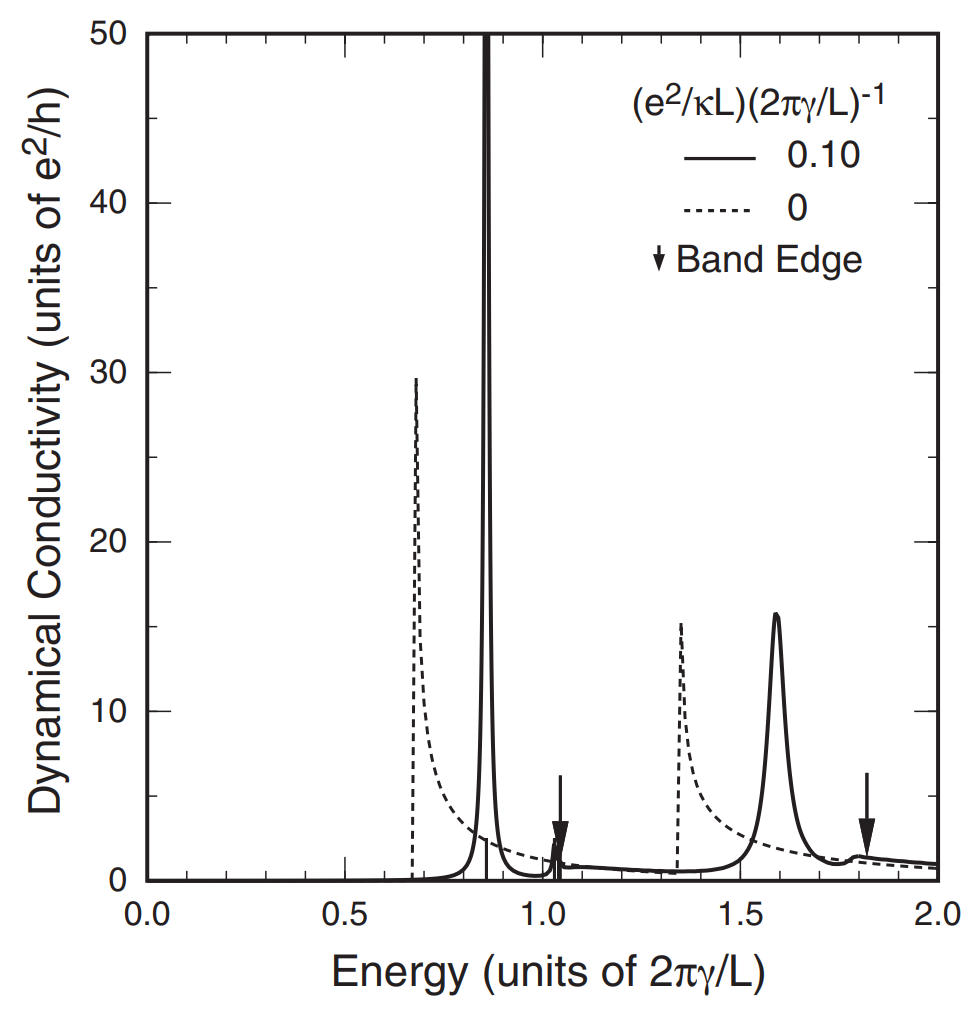
\includegraphics[scale=0.4]{images/chapter_optical_props/ando_suppression}
 	\caption{Ando figure showing suppression of states. Reproduced and modified from Ref \cite{ando2005theory}.}
 	\label{fig:ando_suppression}
 \end{figure}

{\color{red} UNFINISHED} Strength of Coulomb interactions parameterized by the expression $(e^2 \kappa L)/(2 \pi \gamma/L) $ \cite{ando1997excitons}. Here,$e$ is charge of an electron, $\gamma$ is a free parameter, $L = |\vec{C_h} |$, $\kappa$ statis dielectric constant used to account for screening effects. Coulomb interactinos effectively suppress the oscillator strengths of the free electron continuum states. Strength transferred to lowest energy bound states of excitons. Band edge also shifted as a result of coulomb interaction \cite{ando1997excitons}. In fact, it has been experimentally demonstrated that all optical excitations in carbon nanotubes lead to the direct creation of excitons \cite{wang2005optical}. 



\subsection{Exciton Binding Energies}


Binding energies on order of hundreds of meV. Means that excitons are quite stable at room temperature. Quite unusual because in contrast, well-known semiconductors such as GaAs only exhibit excitons with binding energies typically less than 10 meV. Samples have to be cooled down to low temperatures in order to easily observe exciton resonances \cite{liang1970excitons}. Unusual dominance of excitons in electronic structure gives opportunity to study physics of excitons.



\begin{figure}[h]
	\centering
	\includegraphics[scale=0.7]{example-image-a}
	\caption{Figure of GaAs absorbance at low-T and high-T to show weak binding energy of excitons. Next to this is a figure of  (6,5) absorbance at room temperature}
	\label{fig:gaas_vs_cnt_absorbance}
\end{figure}


\section{Optical Selection Rules}

{\color{red}UNFINISHED} Selection rules dictate the optical transitions that can occur. Such optical processes depend upon the conservation of both energy and angular momentum \cite{weismanKonoBook}. The notation E$_{ij}$ denotes an inter-band transition between the valence sub-band $i$ and the conduction sub-band $j$ \cite{weismanKonoBook}. Incident light polarized parallel to carbon nanotube axial direction excites transitions where $i=j$ \cite{weismanKonoBook}. Incident light polarized perpendicular to the nanotube axial direction can only excite optical transitions where $|i-j|=1$ \cite{weismanKonoBook}. 


\begin{figure}[H]
	\centering
	\begin{subfigure}{\textwidth}
		\centering
		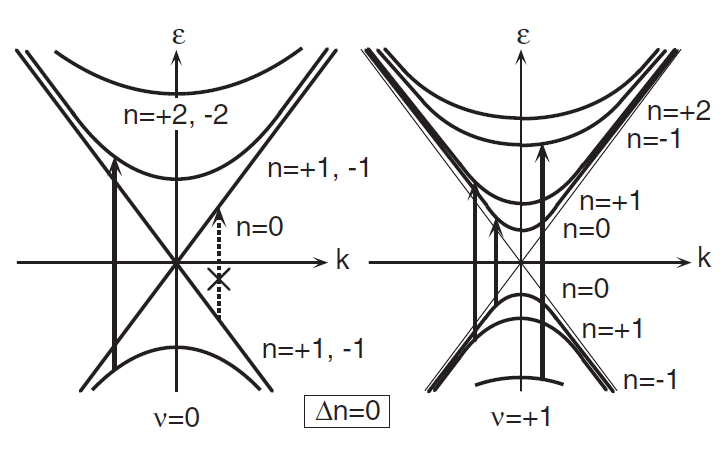
\includegraphics[scale=0.7]{images/chapter_optical_props/selection_rules_1.png}
		\caption{Selection Rules for Parallel case.}
	\end{subfigure}
	\begin{subfigure}{\textwidth}
		\centering
		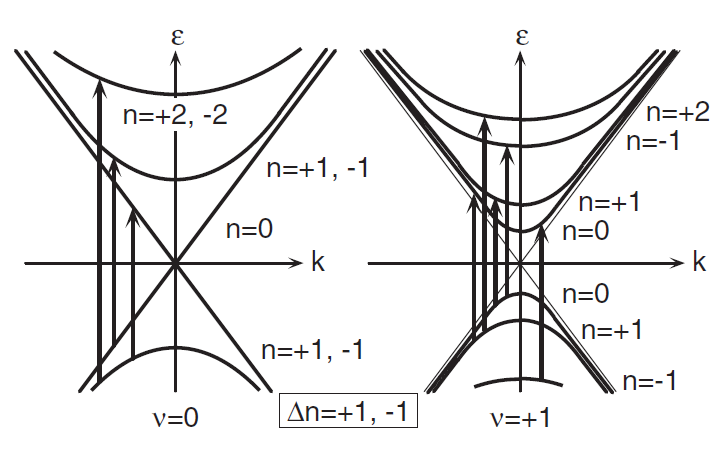
\includegraphics[scale=0.7]{images/chapter_optical_props/selection_rules_2.png}
		\caption{Selection rules for perpendicular case}
	\end{subfigure}
	\caption{Selection rules. Reproduced from Ref \cite{ando2005theory}.}
	\label{fig:selection_rules}
\end{figure}

\section{Summary}

Different species are distinguishable using a set of indices (m,n). Can distinguish between metallic and semiconducting nanotubes with this definition. 1-D character of nanotubes establishes strong quantum confinement, bolsters the role of electron-electron interactions. Strong coulomb interactions lead to excitons with very high binding energies. Theory also shows that excitonic resonances diminish the density of states associated with the free electron continuum.